\PassOptionsToPackage{dvipsnames,table}{xcolor}
\documentclass[10pt]{beamer}
\usepackage{Cours}

\begin{document}

\input{\detokenize{/home/fenarius/Travail/Cours/NSITerminale/docs/commun/MacrosCours.tex}}
\setcounter{numchap}{6}


\pythonmode
\newcommand{\SL}{\cnum Strcutures de données linéaires}


\newcommand{\maillon}[3]{
	\begin{tabular}{|p{0.2cm}|p{0.2cm}|}
		\hline
		\rnode{#2}{#1} & \rnode{#3}{\phantom{$e_0$}} \\
		\hline
	\end{tabular}
}


% Définition d'une structure de données
\begin{frame}{\SL}
	\mframe{\SL}
	\begin{alertblock}{Définition : structure de données}
		\begin{itemize}
			\item<1-> En informatique, une \textcolor{blue}{structure de données} est une façon d'organiser, de gérer et de stocker des données permettant d'accéder et de modifier ces données de façon efficace. \\
			      \onslide<2->\textcolor{OliveGreen}{\small Les listes de Python sont une structure de données.}
			\item<3-> L'\textcolor{blue}{interface} de la structure de données est l'ensemble des opérations accessibles à un utilisateur de la structure de données. \\
			      \onslide<4->\textcolor{OliveGreen}{\small {\tt append} qui permet d'ajouter un élément à la fin d'une liste de Python fait partie de l'interface des listes}\\
			\item<5-> L'\textcolor{blue}{implémentation} de la structure de données est la façon dont elle est représentée et codée en mémoire et n'est pas forcément accessible à l'utilisateur. Cependant, la complexité des opérations de l'interface est généralement fournie.\\
			      \onslide<6>\textcolor{OliveGreen}{\small Nous ne savons pas comment sont représentées ou codées les listes de Python, mais nous savons que par exemple la copie d'une liste est une opération en $O(n)$}
		\end{itemize}
	\end{alertblock}
\end{frame}


% Exemple
\begin{frame}{\SL}
	\mframe{\SL}
	\begin{exampleblock}{Exemple}
		On considère l'instruction suivante en Python : \\
		{\tt res = \{"a":2, "e":9, "i" : 5, "o" : 1, "u" : 7 \}}
		\begin{itemize}
			\item<1-> Quelle est la structure de donnée utilisée ici ?
			\item<2-> Quel élément de l'interface permet de parcourir les valeurs stockées 2,9,5,1 et 7 ?
			\item<3-> Comment ajouter la paire {\tt "y":0} à cette structure de données ?
			\item<4-> Savez-vous comment est implémentée cette structure de données en Python ?
		\end{itemize}
	\end{exampleblock}
\end{frame}

% Interface et implémentation
\begin{frame}{\SL}
	\mframe{\SL}
	\begin{alertblock}{Caractérisation par l'interface}
		\begin{itemize}
			\item<1-> La différence entre \textcolor{blue}{interface} et \textcolor{blue}{implémentation} est fondatamentale et doit être bien comprise. En effet une même structure de données peut avoir plusieurs implémentations. C'est comme par exemple un téléviseur, on retrouve toujours la même interface (la télécommande) mais l'implémentation peut être différente (tube cathodique, écran plasma, lcd, led, \dots).
			\item<2-> Lorsqu'on définit un \textit{cahier des charges} pour une structure de données (ensemble des données et opérations possibles), on définit ce qu'on appelle un \textcolor{blue}{type abstrait de données}.  Ainsi, une structure de données peut être vue comme une implémentation d'un type abstrait de données.
		\end{itemize}
	\end{alertblock}
\end{frame}

% Piles : approche sémantique
\begin{frame}{\SL}
	\mframe{\SL}
	\begin{alertblock}{Piles}
		\begin{itemize}
			\item<1-> Au niveau sémantique, une \textcolor{blue}{pile} est semblable à une pile d'objet dans la vie de tous les jours.
			      \onslide<2->{\begin{center}
				      \hspace{-2.5cm} \onslide<6->{\rnode{emp}{\framebox[1cm]{\tt elt}}} \qquad \qquad \qquad \qquad \qquad \onslide<9->{\rnode{dep}{\framebox[1cm]{\tt elt}}} \\
				      \begin{tabular}{|p{1cm}|c}
					      \cline{1-1}
					      \rnode{sommet}{\tt elt4} & \onslide<4->{$\leftarrow$ \textcolor{blue}{sommet}} \\
					      \cline{1-1}
					      {\tt elt3}               &                                                     \\
					      \cline{1-1}
					      {\tt elt2}               &                                                     \\
					      \cline{1-1}
					      {\tt elt1}               &                                                     \\
					      \cline{1-1}
				      \end{tabular}}
				      \onslide<6->{\ncangle[angleB=90, armB=0,offsetB=-0.1cm,linestyle=dashed]{->}{emp}{sommet}}
				      \onslide<7->{\rput(-4.2,1.4){{\footnotesize \textcolor{blue}{empiler}}}}
				      \onslide<9->{\ncangle[angleB=90, armB=0,nodesepA=-1cm,linestyle=dashed]{<-}{dep}{sommet}}
				      \onslide<10->{\rput(-1.8,1.4){{\footnotesize \textcolor{blue}{dépiler}}}}
			      \end{center}
			\item<3->{L'élément situé en haut de la pile s'appelle le \textcolor{blue}{sommet}.}
			\item<5-> Empiler signifie ajouter un élément au sommet de la pile
			\item<8-> Dépiler signifie retirer l'élément situé au sommet de la pile
			\item<11-> Ainsi le premier élément entré dans la pile sera aussi le dernier à en sortir, on dit qu'une pile est une structure \textcolor{blue}{\sc lifo} \textit{Last In First Out}
		\end{itemize}
	\end{alertblock}
\end{frame}


% Piles
\begin{frame}{\SL}
	\mframe{\SL}
	\begin{alertblock}{Piles comme structures de données}
		L'interface d'une structure de données Pile se limite donc aux opérations suivantes :
		\begin{itemize}
			\item<2-> \textcolor{blue}{\tt est\_vide()} qui renvoie un booléen indiquant si la pile est vide ou non.
			\item<3-> \textcolor{blue}{\tt empiler()} qui ajoute un élément au sommet de la pile.
			\item<4-> \textcolor{blue}{\tt depiler()} qui retire l'élément situé au sommet (cela n'est possible que si la pile n'est pas vide).
		\end{itemize}
	\end{alertblock}
	\onslide<5->{
		\begin{block}{Utilisation}
			En dépit de sa simplicité, cette structure de données a de nombreuses applications en informatique : pile d'appel récursif, pile d'évaluation d'une expression, \dots
		\end{block}}
\end{frame}

% Piles : EX1
\begin{frame}{\SL}
	\mframe{\SL}
	\begin{exampleblock}{Manipulation de piles}
		\begin{itemize}
			\item<2-> On considère la pile : {\tt P = |"A","L","I","X">} (le sommet est {\tt "X"}). Quelle suite d'opération permet d'obtenir {\tt P=|"A","L","E","X">} ?
			\item<3-> Un programmeur décide d'utiliser une pile afin de stocker une réponse entrée au clavier. Chaque caractère tapé doit être empiler. Traduire en terme d'opérations sur cette pile les actions suivantes :
			      \begin{enumerate}
				      \item<4-> Appuie sur la touche "o"
				      \item<5-> Appuie sur la touche "i"
				      \item<6-> Appuie sur la touche \framebox{$\longleftarrow$} (\textit{backspace})
				      \item<7-> Appuie sur la touche "k"
			      \end{enumerate}
		\end{itemize}
	\end{exampleblock}
\end{frame}

% Piles : EX2
\begin{frame}{\SL}
	\mframe{\SL}
	\begin{exampleblock}{Manipulation de piles}
		Au jeu des tours des Hanoï, on gère les trois tours {\tt T1, T2 et T3} à l'aide de trois piles.
		\begin{enumerate}
			\item<2-> Quel est le contenu de chacune des piles dans la situation ci-dessous ? (un disque est réprésenté dans la pile par sa taille)
			      \begin{center}
				      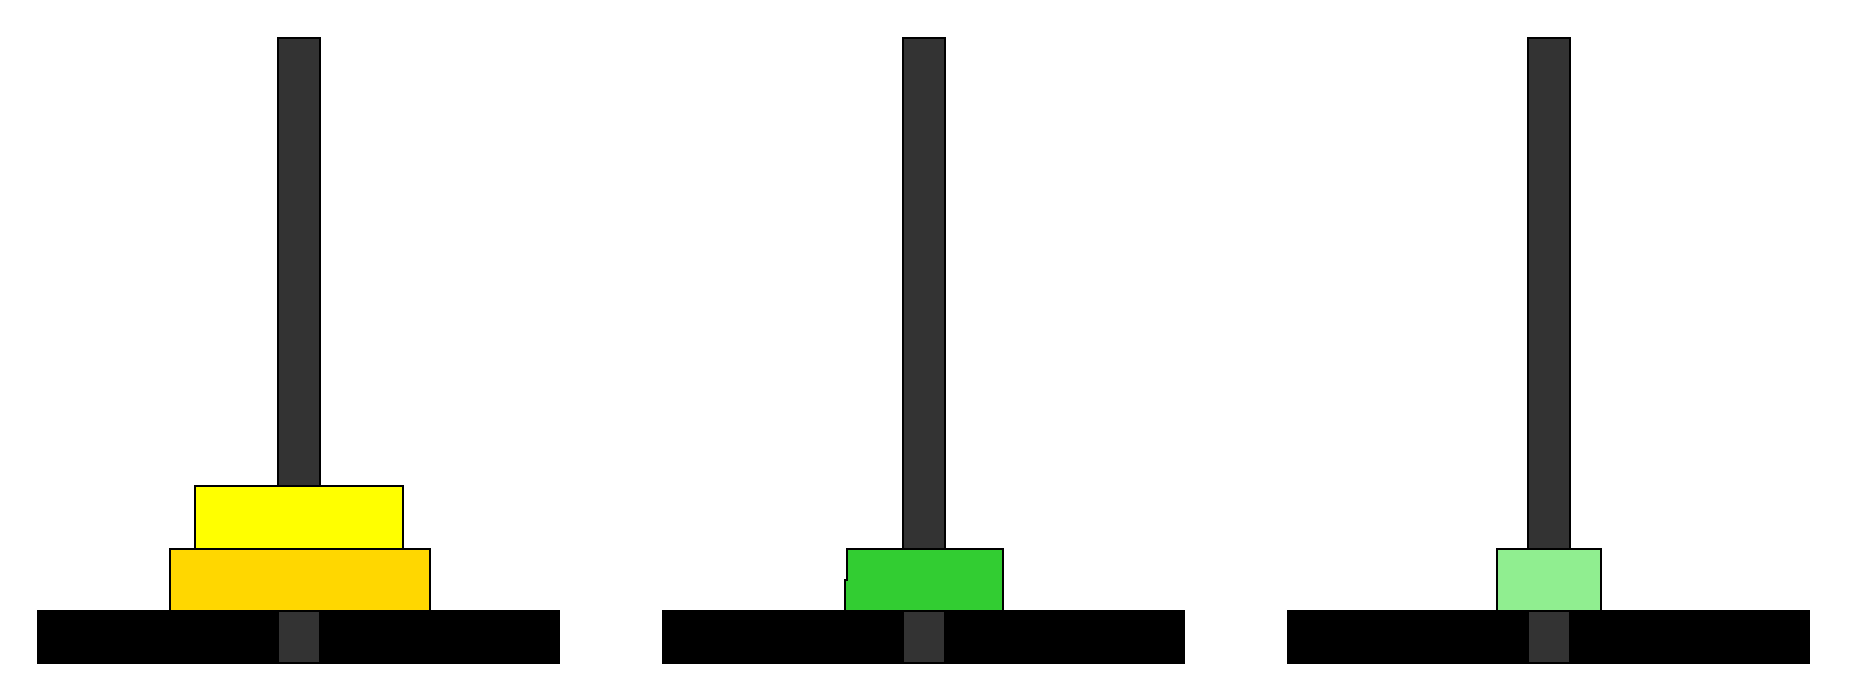
\includegraphics[scale=0.14]{hanoi_dep.eps}
			      \end{center}
			\item<3-> Ecrire les opérations permettant de passer la situation précédente à celle ci-dessous :
			      \begin{center}
				      \includegraphics[scale=0.18]{hanoi_fin.eps}
			      \end{center}
		\end{enumerate}
	\end{exampleblock}
\end{frame}



% Files : approche sémantique
\begin{frame}{\SL}
	\mframe{\SL}
	\begin{alertblock}{Files}
		\begin{itemize}
			\item<1-> Au niveau sémantique, une \textcolor{blue}{file} est semblable à une file d'attente dans la vie de tous les jours.
			      \onslide<2->{\begin{center}
				      \onslide<4->{\rnode{enf}{\framebox[1cm]{\tt elt}}}  \hspace{1cm}
				      \begin{tabular}{|p{1cm}|p{1cm}|p{1cm}|p{1cm}|}
					      \hline
					      \rnode{in}{\tt elt4} & {\tt elt3} & {\tt elt2} & \rnode{out}{\tt elt1} \\
					      \hline
				      \end{tabular}
				      \hspace{1cm} \onslide<9->{\rnode{def}{\framebox[1cm]{\tt elt}}}
				      }
				      \onslide<5->{\ncline[linestyle=dashed,nodesepB=0.2cm]{->}{enf}{in}}
				      \onslide<6->{\naput{{\footnotesize \textcolor{blue}{enfiler}}}}
				      \onslide<9->{\ncline[linestyle=dashed,nodesepA=0.4cm]{->}{out}{def}}
				      \onslide<10->{\naput{{\footnotesize \textcolor{blue}{défiler}}}}
			      \end{center}
			\item<3-> Enfiler signifie ajouter un élément en fin de file
			\item<7-> Défiler signifie retirer l'élément situé au début de la file.
			\item<11-> Ainsi le premier élément entré dans la file sera aussi le premier à en sortir, on dit qu'une file est une structure \textcolor{blue}{\sc fifo} \textit{First In First Out}
		\end{itemize}
	\end{alertblock}
\end{frame}



% Files
\begin{frame}{\SL}
	\mframe{\SL}
	\begin{alertblock}{Files comme structures de données}
		L'interface d'une structure de données File se limite donc aux opérations suivantes :
		\begin{itemize}
			\item<2-> \textcolor{blue}{\tt est\_vide()} qui renvoie un booléen indiquant si la file est vide ou non.
			\item<3-> \textcolor{blue}{\tt enfiler(element)} qui ajoute un élément à la fin de la file.
			\item<4-> \textcolor{blue}{\tt defiler()} qui retire l'élément situé au début de la file (cela n'est possible que si la file n'est pas vide).
		\end{itemize}
	\end{alertblock}
	\onslide<5->{
		\begin{block}{Utilisation}
			Comme pour les piles, cette structure de données a de nombreuses applications en informatique : file d'attente d'une imprimante, simulation de files d'attentes réelles, \dots
		\end{block}}
\end{frame}

% Piles : EX1
\begin{frame}{\SL}
	\mframe{\SL}
	\begin{exampleblock}{Manipulation de files}
		\begin{itemize}
			\item<2-> On considère la file : {\tt F = >"E","L","S","A">}. Quelle suite d'opération permet d'obtenir {\tt F= >"N","O","E","L">} ?
			\item<3-> On simule la file d'attente d'une imprimante à l'aide d'une file. A quelle opération sur cette file correspond l'envoie d'une nouvelle impression ? La fin de l'impression en cours ? Dans quel ordre seront effectuées les impressions ?
		\end{itemize}
	\end{exampleblock}
\end{frame}

% Listes : approche sémantique
\begin{frame}{\SL}
	\mframe{\SL}
	\begin{alertblock}{Listes}
		\begin{itemize}
			\item<1-> Au niveau sémantique, une \textcolor{blue}{liste} est suite finie d'éléments (avec répétition éventuelle) on peut noter une liste : $e_0, e_1, \dots, e_n$.
			\item<2-> L'interface d'une liste contient généralement les éléments suivants :
			      \begin{itemize}
				      \item<3-> Un constructeur permettant de créer la liste vide.
				      \item<4-> Une opération renvoyant un booléen suivant que la liste soit vide ou non.
				      \item<5-> Une opération permettant d'ajouter un élément en début (ou en fin) de liste.
				      \item<6-> Une opération renvoyant le premier élément de la liste (on dit la \textcolor{blue}{tête} de la liste).
				      \item<7-> Une opération renvoyant la \textcolor{blue}{queue} de la liste, c'est à dire la liste privée de sa tête.
				      \item<8-> Une opération permettant d'accéder à un élément de la liste par son index.
			      \end{itemize}
			\item<9-> Deux implémentations des listes sont généralement utilisées :
			      \begin{itemize}
				      \item<10-> Par un tableau (éléments contigues en mémoire)
				      \item<11-> Par une liste chainée (chaque élément contient alors un lien vers le suivant)
			      \end{itemize}
		\end{itemize}
	\end{alertblock}
\end{frame}

% Listes : ambiguités
\begin{frame}{\SL}
	\mframe{\SL}
	\begin{block}{\textcolor{yellow}{\danger} \; Ambiguité}
		\begin{itemize}
			\item<1-> Le terme \textcolor{blue}{liste} devient ambigüe, en effet c'est à la fois le nom du type abstrait de données que nous venons de définir mais aussi celui d'une structure de données existante en Python.
			\item<2-> D'autres part, pour amplifier encore cette ambiguité, le terme \textit{liste chaînée}, est parfois abrégé en liste, alors qu'il s'agît d'une implémentation possible et pas du type abstrait de données défini plus haut.
		\end{itemize}
	\end{block}
\end{frame}

%Listes : implémentation en Python
\begin{frame}
	\mframe{\SL}
	\begin{block}{Python et le {\sc tad} liste}
		\begin{itemize}
			\item<1->En Python, le {\sc tad} liste est implémenté sous forme de tableau, c'est à dire que les éléments d'une liste de Python sont \textcolor{blue}{contigues} en mémoire :
			      \begin{center}
				      \begin{tabular}{l|p{0.2cm}|p{0.2cm}|p{0.2cm}|p{0.2cm}|p{0.2cm}|p{0.2cm}|p{0.2cm}|}
					      \cline{2-8}
					      Eléments                    & $e_0$                            & $e_1$                            & $e_2$                            & $e_3$                            & $e_4$                            & $e_5$                            & \dots                            \\
					      \cline{2-8}
					      \multicolumn{1}{c}{ }       & \multicolumn{1}{c}{$\downarrow$} & \multicolumn{1}{c}{$\downarrow$} & \multicolumn{1}{c}{$\downarrow$} & \multicolumn{1}{c}{$\downarrow$} & \multicolumn{1}{c}{$\downarrow$} & \multicolumn{1}{c}{$\downarrow$} & \multicolumn{1}{c}{$\downarrow$} \\
					      \multicolumn{1}{c}{Indices} & \multicolumn{1}{c}{0}            & \multicolumn{1}{c}{1}            & \multicolumn{1}{c}{2}            & \multicolumn{1}{c}{3}            & \multicolumn{1}{c}{4}            & \multicolumn{1}{c}{5}            & \multicolumn{1}{c}{6}            \\
				      \end{tabular}
			      \end{center}
			\item<2-> L'autre implémentation que nous avons évoquée (celle par les listes chaînées) peut être importé à partir du module {\tt collections} ou écrite par exemple à l'aide de la {\sc poo}. Dans ce cas, les éléments d'une liste ne sont plus contigues en mémoire mais chaque élément doit aussi contenir un lien vers son suivant dans la liste :
			      \begin{center}
				      \rnode{head}{\phantom{Y}}  \quad \maillon{$e_0$}{v0}{p0} \  \maillon{$e_1$}{v1}{p1}  \maillon{$e_2$}{v2}{p2}  \maillon{$e_3$}{v3}{p3}  \maillon{$e_4$}{v4}{p4} \maillon{$e_5$}{v5}{p5}\ncline[nodesepB=0.25cm]{->}{p0}{v1}
				      \ncline[nodesepB=0.25cm]{->}{p1}{v2}
				      \ncline[nodesepB=0.25cm]{->}{p2}{v3}
				      \ncline[nodesepB=0.25cm]{->}{p3}{v4}
				      \ncline[nodesepB=0.25cm]{->}{p4}{v5}
			      \end{center}
		\end{itemize}
	\end{block}
\end{frame}

%Listes : avantages et inconvenients des implementations
\begin{frame}
	\mframe{\SL}
	\begin{block}{Avantages et inconvénients de ces implémentations}
		Ces deux implémentations ont des conséquences importantes en terme de complexité des opérations mais aussi d'occupation mémoire :
		\begin{itemize}
			\item<1-> Sous forme de liste chaînée, l'occupation mémoire est plus importante (on stocke en plus de l'élément le lien vers l'élément suivant).
			\item<2-> Accéder à un élément sous forme de tableau est direct alors que pour une liste chaînée il faut avoir parcouru au préalable tout ceux qui le précèdent depuis la tête.
			\item<3-> L'insertion d'un élément dans un tableau oblige à décaler ceux qui le suivent alors que l'opération est directe en liste chaînée.
			\item<4-> L'ajout d'un élément en fin de liste oblige à agrandir le tableau si la taille initialement prévue est dépassée alors qu'avec une liste cela ne pose pas de problèmes.
		\end{itemize}
	\end{block}
\end{frame}

\begin{frame}
	\mframe{\SL}
	\begin{alertblock}{Choix d'une structure de données}
		En conclusion : on utilisera
		\begin{itemize}
			\item<2-> Un tableau (et donc une liste de Python) lorsque la taille des données est connu par avance  et/ou lorsqu'on a besoin d'accéder aux éléments par leur indice rapidement.
			\item<3-> Une liste chainée (module {\tt deque}) pour les structures à taille variable et/ou lorsqu'on a besoin d'insérer ou de supprimer les éléments situés au debut ou à la fin.
		\end{itemize}
	\end{alertblock}
\end{frame}

\end{document}